%; whizzy chapter
% -initex iniptex -latex platex -format platex -bibtex jbibtex -fmt fmt
% 以上 whizzytex を使用する場合の設定。

%     Tokyo Debian Meeting resources
%     Copyright (C) 2007 Junichi Uekawa

%     This program is free software; you can redistribute it and/or modify
%     it under the terms of the GNU General Public License as published by
%     the Free Software Foundation; either version 2 of the License, or
%     (at your option) any later version.

%     This program is distributed in the hope that it will be useful,
%     but WITHOUT ANY WARRANTY; without even the implied warranty of
%     MERCHANTABILITY or FITNESS FOR A PARTICULAR PURPOSE.  See the
%     GNU General Public License for more details.

%     You should have received a copy of the GNU General Public License
%     along with this program; if not, write to the Free Software
%     Foundation, Inc., 51 Franklin St, Fifth Floor, Boston, MA  02110-1301 USA

%  preview (shell-command (concat "evince " (replace-regexp-in-string "tex$" "pdf"(buffer-file-name)) "&"))
% 画像ファイルを処理するためにはebbを利用してboundingboxを作成。
%(shell-command "cd image200708; ebb *.png")

%%ここからヘッダ開始。

\documentclass[mingoth,a4paper]{jsarticle}
\usepackage{monthlyreport}

% 日付を定義する、毎月変わります。
\newcommand{\debmtgyear}{2007}
\newcommand{\debmtgdate}{15}
\newcommand{\debmtgmonth}{9}
\newcommand{\debmtgnumber}{32}


\begin{document}

\begin{titlepage}

% 毎月変更する部分, 本文の末尾も修正することをわすれずに

 第\debmtgnumber{}回 東京エリア Debian 勉強会資料

\vspace{2cm}

\begin{minipage}[t]{0.6\hsize}
\vspace{-2cm}
{\fontsize{60}{60}
{\gt
\color{dancerdarkblue}
東京エリア \\
デビアン \\
勉強会
}}
\end{minipage}
\begin{minipage}[b]{0.4\hsize}
\hspace{-1cm}
\includegraphics[width=9cm]{image200502/openlogo-nd.eps}
\end{minipage}

\vspace{3cm}
\hfill{}Debian勉強会幹事 上川 純一\\
\hfill{}\debmtgyear{}年\debmtgmonth{}月\debmtgdate{}日

\thispagestyle{empty}
\end{titlepage}

\dancersection{Introduction}{上川 純一}


今月のDebian勉強会へようこそ。
 これからDebianのあやしい世界に入るという方も、すでにどっぷりとつかってい
 るという方も、月に一回Debianについて語りませんか?

 目的として次の二つを考えています。

 \begin{itemize}
 \item メールではよみとれない、もしくはよみとってられないような情報につ
       いて情報共有する場をつくる
 \item Debianを利用する際の情報をまとめて、ある程度の塊として整理するた
       めの場をつくる
 \end{itemize}

 Debianの勉強会ということで究極的には参加者全員がDebian Packageをがりがり
 と作るスーパーハッカーになった姿を妄想しています。

 Debianをこれからどうするという能動的な展開への土台としての空間を提供し、
 情報の共有をしたい、というのが目的です。


\newpage

\begin{minipage}[b]{0.2\hsize}
 \colorbox{dancerlightblue}{\rotatebox{90}{\fontsize{80}{80} 
{\gt \color{dancerdarkblue}デビアン勉強会}}}
\end{minipage}
\begin{minipage}[b]{0.8\hsize}
\hrule
\vspace{2mm}
\hrule
\setcounter{tocdepth}{1}
\tableofcontents
\vspace{2mm}
\hrule
\end{minipage}

\dancersection{事前課題}{岩松 信洋}

今回の事前課題は
「あなたがDebianで使っている MTA のこだわりの設定」もしくは「Debian 
で利用しているこんな便利な/楽しいメッセージツールあるいは日頃使っていて
気にかかるメッセージ関連ソフトのこの部分」
というタイトルで200-800文字程度の文章を書いてください。というものでした。
その課題に対して下記の内容を提出いただきました。

\subsection{やまねひできさん}

\begin{itemize}
\item その昔、postfix + fml で運用をしていたところ、unstable の postfix 
パッケージを入れたら postfix にバグがあって無効な directive を書いたら踏み台
にされたことがありました orz (普通なら無視されるだけなのに、なぜかリレーを受け付
けてしまうのでした。リレーチェックの CGI のページなどで確認はしたのですが…いまだ
に受け付けた理由は不明)

\item そういや fml って fml8 は本当に出てくるのでしょうか。いまだと mailman 
が標準メーリングリストドライバなのかな。

\item qmail は捨てたいのですが、いまだに使いたい人とかいるんですよね。ある blog 
でソースから入れていていちいちパッケージ入れなきゃいけない、なんてことが書いてあった
ので apt-get build-dep qmail-src で必要そうなパッケージ入れれば良いのに、
と書いたら逆切れされたのもいい記憶です ;-)

\item ある人は Debian をインストールして最初にするのは nano ではなく vi 
をデフォルトエディタにすることと exim を削除して postfix を入れることと言っていましたが、
私も postfix を入れています。理由は単に昔触ったことがあって勘が効くだろうから、というだけ
ですが。

\item 複数 MTA を同時に入れられると良いですよね。

\item spam 対策は非常に大変そうです。spamassassin は入れて手元で運用した事がありますが、
CPU を非常に喰うので中古ノートPCでは問題です。どういう対応が spam 対策として一番良いので
しょうか?
\end{itemize}

\subsection{本庄さん}
MTAにはPostfixを利用しています。

MTAで特にこだわった設定は行っていませんが、MDAにprocmailを使用し、
ここから添付メールの自動圧縮などを設定したりしています。

\subsection{濱野さん}
\subsubsection{あなたがDebianで使っている MTA のこだわりの設定}
qmail から脱却できないひとりです、exim に超期待。
qmail はちょこっと弄ってエンベロープ To が使用しているメールアドレスじゃ
なかったらその場で SMTP エラーを返してTCP コネクションを切る、というよ
うなことをやっています。backscatter なメールを撒かなくて良いのと spam
が減っているような気分になります。

\subsubsection{Debian で利用しているこんな便利な/楽しいメッセージツール}
最近 ejabberd で遊んでます。ejabberd は Erlang で書かれた jabber サーバー
です。最新の erlang 実行環境 + openssl + ejabberd をソースからコンパイ
ルすると openssl の兼ね合いではまるのですが(古い Erlang だと動く)、
debian package はサクッと動作するのでお手軽です。


\subsection{山本浩之さん}
\subsubsection{日頃使っていて気にかかるメッセージ関連ソフトのこの部分}

まず、KSirc について。
KSirc を ISO-2022-JP (JIS) でつかっていると、
以下の (?? 7e) の文字コードのもの 67 個の後に続く文字列が化けます。

蔭 応 改 萱 棄 京 屈 捲 向 込 刷 時 周 償 飾 裾 線 憎 只 寵
逓 到 入 麦 美 服 朋 満 癒 璃 聯 傲 辨 咨 圉 奩 屓 廏 悚 戛
撼 暼 棍 檣 沾 滌 燼 珱 癰 磬 筐 紆 缺 腋 苙 蕈 蝙 襞 譫 蹊
迸 錮 陞 顰 髷 鵈 龠

↓こんなかんじ
\begin{commandline}
<yamamoto> 時?慌修韻襪里?福??
<yamamoto> 周???
\end{commandline}

「設定→KSirc を設定→色→強調→kSirc の色コードを削除」
にチェックを入れていると確実に化けるのですが、
チェックを外していても時々化け始めます。

再現条件がいまいち分からず、それに日本語特有なんで、
BTS にも出しずらいのが難点です。

あと、Icedove について。
どうでも良いようなことですが、sid の Icedove のボタンのアイコンが
Thunderbird オリジナルのものと同じなのは気になります(わら
それに、OpenPGP のサインの詳細を知るためのペンアイコンが出ないのも
少々難儀しています

\subsection{前田 耕平さん}
\subsubsection{あなたがDebianで使っている MTA のこだわりの設定}

自宅環境では、一つ一つは特に変わった設定はしていませんが、
メールを内部のメールサーバ(B)に集約し、どのクライアントを
使ってもメールを見られるようにしています。

記号の説明と使用しているソフト
\begin{description}
\item[A] 外向けMTA(Postfix)
\item[B] 内部メールサーバ 
	(MTA \& MDU \& MUA)(Postfix \& Courier-IMAP \& Fetchmail)
\item[C] 他用途のサーバ (ssmtp)
\item[D] クライアント用PC(Postfix)
\end{description}

メール送信時
\begin{itemize}
\item C or D → B → A → Internet
 メール受信時(外からの自ドメイン)
\item C → B ← A ← Internet
 メール受信時(自宅内での自ドメイン)
\item C → B ← [A|B|C|D]
 メール受信時(ISPのメール)
\item C → B → ISPメールサーバ
\end{itemize}

C, DはBを、BはAをリレー先にし、A, Bでは自ドメイン当てのみBに向けるようにしています。
ISPからのメールをB(内部メールサーバ)で直接fetchmailで取りに行っているので、
SpamAssassinをBでspamdで動かしています。
Cのメールサーバ以外のサーバでは、Postfixでは機能が多すぎるのでssmtpを使っています。
Dのクライアントでssmtpを使わなかったのは、ネットワークから切り離していると、メールが
ローカルキューに貯まらず、消失してしまうためです。

\subsection{小室 文さん}
\subsubsection{あなたがDebianで使っている MTA のこだわりの設定}
Exim 4 と一緒に ClamAV, SpamAssassin, Mailman を動かしています。
ClamAV/SpamAssassinは
\begin{commandline}
/etc/exim4/conf.d/main/02_exim4-config_options
\end{commandline}
に
\begin{commandline}
av_scanner = clamd:/var/run/clamav/clamd.ctl
spamd_address = 127.0.0.1 783
\end{commandline}
と追加。exim4-daemon-heavyに感謝。

後はMailmanのaliasをEximが自動生成してくれるから便利だなとか。
\begin{commandline}
  mailman_router:
    driver = accept
    require_files = MAILMAN_HOME/lists/$local_part/config.pck
    local_part_suffix_optional
    local_part_suffix = -bounces : -bounces+* : \
                        -confirm+* : -join : -leave : \
                        -owner : -request : -admin
    transport = mailman_transport
\end{commandline}

\subsection{岩松}

\subsubsection{あなたがDebianで使っている MTA のこだわりの設定}
家で動いているサーバーの MTA は Postfix を使っています。
ライセンスや設定方法などを考えると自動的に Postfix になってしまいました。
特にこだわりの設定は行っていません。

\subsubsection{Debian で利用しているこんな便利な/楽しいメッセージツールあるいは日頃使っていて
気にかかるメッセージ関連ソフトのこの部分}
普段使っているのは ekiga です。一時は家に sip サーバーを立ち上げて遊んでいました。
最近は USB カメラにはまっているので、画像転送用に使っていたりします。

%%% trivia quiz
\dancersection{Debian Trivia Quiz}{岩松 信洋}

ところで、みなさん Debian 関連の話題においついていますか?Debian関連の話
題はメーリングリストをよんでいると追跡できます。ただよんでいるだけではは
りあいがないので、理解度のテストをします。

今回の出題範囲は\url{debian-devel@lists.debian.org} に投稿された内容からです。

\subsection{問題}

\santaku
{Albert Einstein が作った Debian ベースのディストリビューションは何か}
{ice linux}
{fantasy linux}
{fire linux}
{A}

\santaku
{そしてこのAlbert Einstein が debian-devel で質問した内容は何でしょう}
{なぜ Internet Explorer が Debian にないのですか。}
{なぜ Opera が Debian にないのですか。}
{なぜ Safari が Debian にないのですか。}
{B}

\santaku
{Luk Claes が RCバグについて提案したのはどのような内容か}
{RCバグが出たパッケージのメンテナへのペナルティを考える提案}
{RCバグの 0-day NMU についての提案}
{RCバグをいかにして無視するか、という HowTo.}
{B}

\santaku
{packages.debian.orgにいろいろ新機能が追加されました。どのような機能が追加されましたか}
{メールフォワード機能}
{カルマ付加機能}
{Webからパッケージ乗っ取り機能}
{A}

\dancersection{最近のDebian関連のミーティング報告}{岩松 信洋}


\subsection{東京エリアDebian勉強会31回目報告}
% (query-replace-regexp "<.*?>" "")
% (query-replace-regexp "^[ 	]*" "")

東京エリアDebian勉強会参加報告。8月の第31回東京エリアDebian勉強会を実施し
ました。

 今回の参加者は 小室文さん、根岸心さん、後藤正徳さん、前田耕平さん、やまねひできさん、
濱野さん、たかやさん、 すずきくにおさん、荒木(靖)さん、森田さん、林淳哉さん、荒木淳さん、
さとうのりあきさん、岩崎修さん、奥野由紀さん、 北原さん、uchiyama toru さん、碇永志さん、 
岩松さん、あけどさん、野首さん、David Smithさん、小林さん、でんさん、上川の25人でした。

まず、クイズを今回も実施しました。 今回はDWNが出ていないので、
debian-devel-announce の内容から出題しました。 
最後までのこった4人に豪華景品が渡されました。

最近のイベントの報告として、 OSC-Kansai について たかやさんが報告しました。 
関西の勢いというものをみんなで感じたのではないでしょうか?

\url{cdn.debian.or.jp} について荒木さんが発表しました。 
\url{cdn.debian.or.jp} をしっている人はおおかったようですが、
仕組みについてはよくしらない人が ほとんどだったので、おもしろかったとおもいます。
意外とシンプルですね。荒木さん的には debtorrent,apt-torrentが気になるようです。 

最後に事前課題の紹介をしました。
はまった話、多かったです。

最後に 上川さんが Debian GNU/kFreeBSD で ruby のアプリケーション apt-listbugs
が正常に動かないというバグ報告を受けたため Debian GNU/kFreeBSD をインス
トールしてみました、という報告をしました。

今回の宴会は  はなの舞 荻窪西口店 にて開催、終電までみんなで宴会しました。

\dancersection{Exim 再発見}{小室 文}
\label{debianexim}
\index{exim}
\subsection{intro}
私達の日常ではメールは欠かせないコミュニケーションツールです。
それを実現する為に、導入される MTA( Mail Transfer Agent )は、どのソフトを使ったら
一番コストパフォーマンスが良いか、またどうやったら会社、グループ、個人のニーズに答える事が
出来るか、システム管理者は日夜頭を悩ましているはずです。そして一度導入したメールサーバーの
仕組みは、なかなか別の仕組みに乗り換えるのは、時間と費用がかかり、問題があったとしてもなか
なか移行しづらいという現状もあり、MTAを決めるのは人生でなかなか訪れない大決心の一つである
事は明白です。
MTA の一つ、Exim は Debian の Default MTA と呼ばれながらも、今や Postfix の人気に
すっかり影を潜めて過去の栄光に甘んじているのが現実です。
今日は Exim の歴史、利点・不利点、導入方法を御紹介します。 皆さんの MTA に選ばれなかった
としても、Exim はこういうパッケージなのか!と知って頂ければ幸いです。

\subsection{Eximとは}
Exim\footnote{Exim の名前の由来は EXperimental Internet Mailer (Exim)}
 とは、Unixもしくは Unix like なOSの上で動く Mail Transfer Agent です。Cygwin 
を使えば Windows の上でも動かす事が出来ます。Exim はケンブリッジ大学で 1995 年に Philip Hazel 
さんによって開発されました。\\

\subsection{Exim の歴史}
ケンブリッジ大学では、複数の MTA が動いていて(Sendmail, Smail, PP?などなど)、そんな環境
にうんざりしてたがどうかは不明ですが、Philip Hazel さんは Smail を拡張して MTA を大学のニーズ
に合わせて作ろうと試みました。しかし残念ながら、Smail 拡張はあっさり諦め、Hazel さんはスクラッチ
から MTA を作ろうと試みる事にしました。
その作業が、彼が所属した Computer Sceince の仲間に知れわたり、FTP サーバーを立てられ、配布され
るようになりました。
書いている途中で配布がされるようになった為、正式な Exim 0 もしくは 1 はリリースしていません
(少なくとも Hazel さんはリリース出来なかったと思っているようです)。\\
元々 Sendmail, Smail を触っていた Hazel さんは Sendmail に代わる MTA を作ろうと Exim 
を設計されています。 \\
\begin{tabular}[htb]{|l|l|} \hline
1995年?月 & Exim 開発開始\\ \hline
1995年11月 & 同僚が FTP サーバをつくりパッケージを配布始める。クチコミで広がる\\ \hline
1998年夏 & Perl の正規表現ライブラリーがなかったので作る(PCRE)\\ \hline
1999年3月 & コードネーム Slink の Debian 2.1 リリース。 Exim をディフォルト MTA として起用する \\ \hline
1999年9月 & ケンブリッジ大学で Exim の講座を開始する。 \\ \hline
2000年8月 & コードネーム potato の Debian 2.2 リリース\\ \hline
2002年7月 & コードネーム woody の Debian 3.0 リリース\\ \hline
2004年5月 & ケンブリッジ大学が Exim を正式にサポートすると宣言\\ \hline
2005年6月 & コードネーム sarge の Debian 3.1 リリース\\ \hline
2007年4月 & コードネーム etch のDebian 4.0 リリース\\ \hline
\end{tabular}

\subsection{Exim と Debian の関係}
\subsubsection{現在の Exim のメンテナー}
現在の Exim のメンテナーは
\begin{itemize}
\item Andreas Metzler  \url{ametzler@debian.org}
\item Marc Haber \url{mh@debian.org}
\end{itemize}
です。
Slink で Exim が搭載されるようになる前から、Sendmail や Smail から Exim へ移行を試みる人が沢山いた
ようです。
日本ではマニュアルの日本語可があまり進まず(現在も小数の人達が作業しているのみ)、Slink で Exim が搭載され
たので、移行した、という人が多かったようです。

\subsubsection{なぜ Exim は Debian の Default MTA になったのか!?}

\begin{tabular}[htb]{|l|l|} \hline
1996年09月 & Tim Cutt が Debian で Exim をパッケージとして提供する為に作業を始める \\ \hline
1997年05月 & Exim がunstable に入る by David Sewell \\ \hline
1999年03月 & Slink で Exim をディフォルト MTA として起用する。\\ \hline
\end{tabular}

当時は Postfix、Sendmail, Smail などがあったりましたが、ライセンス問題
\footnote{ライセンス形態:GNU General Public License (GPL)  ver2}
、機能の充実度合などがあり、
Debian の Defualt MTA になったようです。

\subsection{Exim と他の MTA の相違点}

\begin{tabular}[htb]{|l|ccc|} \hline
MTA&ライセンス形態 & メイン製作者 & リリース状態 \\ \hline
qmail&DJBライセンス&D. J. Bernstein& 1997年に出したっきり\\ \hline
Postfix&IBM Public License&Wietse Zweitze Venema&1997年にリリース後、都度都度にリリース \\ \hline
Exim&GPL&Philip Hazel&1995年にリリース後、都度都度リリース \\ \hline
\end{tabular}

{\Large qmail}
\begin{itemize}
\item 1997年からリリースされていない。IPv6 に対応してない。ライセンス形態、導入が難しい
\item 大量メールを配信する場合、セキュリティー面
\end{itemize}

{\Large Postfix}
\begin{itemize}
\item Exim ほど機能の実装がない
\item 移行が簡単、コミュニティーがアクティブ、日本でも使っているユーザーが多い(本も多い)
\end{itemize}

{\Large Exim}
\begin{itemize}
\item 日本語のマニュアルがない
\item コミュニティーがアクティブ、Debian の Default MTA、ライセンス、ドキュメントが豊富(英語)
\end{itemize}

\subsection{Exim の設定方法}
\subsubsection{既存パッケージ一覧}
現在の Debian の stable である etch には以下の Exim 向けパッケージが用意されています。

\begin{tabular}[htb]{|l|l|} \hline
exim4&Exim 4 を簡単にインストールする為にメタパッケージ\\ \hline
exim4-base&全 Exim 4 パッケージ支援パッケージ\\ \hline
exim4-config&Exim 4 設定用パッケージ \\ \hline
exim4-daemon-heavy&追加機能(exiscan-acl含む)を搭載しているデーモンパッケージ\\ \hline
exim4-daemon-light&簡易機能を搭載しているデーモンパッケージ\\ \hline
exim4-daemon-light-dbg&debug用\\ \hline
exim4-dbg&debug用\\ \hline
exim4-dev&ヘッダーファイル用の Exim 4 パッケージ \\ \hline
exim4-doc-html&Exim 4 の html 形式のドキュメントパッケージ\\ \hline
exim4-doc-info& Exim 4 の info 形式のドキュメントパッケージ\\ \hline
\end{tabular}

\subsubsection{インストール方法}

\begin{commandline}
aptitude install exim4 exim4-base exim4-config exim4-daemon-heavy
\end{commandline}
か
\begin{commandline}
aptitude install exim4 exim4-base exim4-config exim4-daemon-light
\end{commandline}
を実行します。

exim-config によって必要な情報入力はプロンプトが出るので指示に従います。 \\
\begin{enumerate}
\item 設定ファイルを分割するか、否か
\item メールの扱いについて(送信サーバの決定)
\item メールドメイン名について
\item 受けつけるメール送信元の IP 制限の決定( IPv6 対応)
\item Virtual Domain の下準備
\item オープンメールの設定
\item ローカルネットワークからの送信の決定
\item ダイヤルアップ時のDNS look upの決定
\item メール形式の決定(mbox/Maildir)
\end{enumerate}

\subsection{Exim のこれから}
 Philip Hazel さんは2007年2月8日付で、9月末に Exim から引退したいと申し出ましたが、
まだ決着はついていません。
すでに Exim を Hazel さんと同等に知っているメンテナーが世界中にいるので、肝はそれを統
括するマネージャーのような人を立てる、という事が大事になってくると思われます。\\
メインで動いている人達は Exim の新機能や、Exim をどのように運営、更新をしていくか 
\url{Exim-future@exim.org} という場所で会議をしようと試みています。\\
Debian では、 Exim 5 がリリースされるタイミングが現在もなお不透明な為、例え Lenny 
が近い未来リリースされる事があっても、その時に Exim 5 が間に合うとは保障出来ません。
日本では私がとりあえずマニュアルの翻訳をしようとExim ユーザー会を作ってみました。\\
\url{https://sourceforge.jp/projects/exim-jp}

\dancersection{あなたの知らないかもしれない apt-xxx}{岩松 信洋}
\label{aptxxx}
\index{apt-xxx}
\subsection{はじめに}
Debian ユーザーは apt がないと生きていけません。
apt-get はみんなが知っているコマンドですが、aptにはいろいろなコマンドが存在します。
今回はあまり知られていない apt-xxx について調べてみました。

\subsection{レベル 小}
勝手にレベルをつけていますが、レベル小 は一般ユーザの方なら知っておいて損はない
というものです。Debian 上での生活を楽にしてくれるかもしれません。

%\subsubsection{apt-howto}
% apt の使い方をまとめた Debian package です。
% 日本語向けのパッケージ apt-howto-ja もあります。

\subsubsection{apt-key}
 apt の GPG鍵リングを制御するフロントエンドです。
 2006年から secure apt が導入された。secure apt は Debian アーカイブの信頼性を
 上げるため導入されたのですが、これには GPG が使われており、一般ユーザーにはちょっと
 難しいかもしれません。しかし、secure apt の GPG のキーは毎年変更されるので、今後使う
 ことがあるかもしれません。
 また、GUI で操作したい人のために 
 gui-apt-key\footnote{http://packages.debian.org/unstable/admin/gui-apt-key} 
 パッケージがあります。
 
\subsubsection{apt-spy}
 ネットワークの情報から最適な apt-line を生成することができるツールです。
 いまは cdn.debian.or.jp があるのでどうでもいいかんじです。

\subsubsection{auto-apt}
 auto-apt は世間では検索用のツールになっています。
 \footnote{ファイル検索用として apt-file というコマンドがあります。}
 \begin{commandline}
 % auto-apt upate
 % auto-apt search stdio.h
 usr/include/stlport/stdio.h     libdevel/libstlport5.1-dev
 usr/include/fcgi_stdio.h        libdevel/libfcgi-dev
 usr/include/H5FDstdio.h libdevel/libhdf5-lam-dev,libdevel/libhdf5-mpich-dev,libdevel/libhdf5-serial-dev
 usr/include/stdio.h     libdevel/libc6-dev
 \end{commandline}
 しかし、auto-apt は コマンド実行時に足りないファイルをパッケージをから探しだし、インストールしてくれるツールだったりします。
 \begin{commandline}
 # auto-apt run ./configure
 \end{commandline}
 

\subsubsection{cron-apt}
 apt-get updte / apt-get uprade を cron で書いているひとをたまに見かけますが、
 cron-apt を使えば、ログに apt の結果をながした|じょうかい設定が可能になります。
 似たような名前で apticron\footnote{http://packages.debian.org/unstable/admin/apticron}
 というパッケージがありますが、これはaptitude の cron-apt 版ではなく 
 セキュリティアップデート情報をメールで送信してくれるツールです。

\subsubsection{apt-proxy / apt-cacher}
 Debian パッケージのキャッシングプロキシを構築するパッケージです。
 例えば、家の中でマシンが数台あり、すべて sid だったとしましょう。特に設定を行ってない場合、
 各マシンは apt-get 毎に ミラーサーバーから Debian パッケージを取得します。
 これは無駄なので、1台だけ Debian パッケージをミラーサーバーから取得し、キャッシュし、他の
 マシンは対象のキャッシュしているパッケージを使ってアップデートを行うようにします。
 これを実現するためのパッケージが apt-proxy / apt-cacher です。
 \begin{figure}[h]
 \begin{center}
使用しない場合

 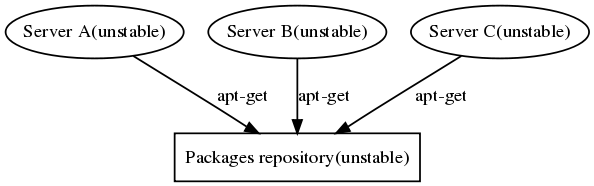
\includegraphics[width=10cm]{image200709/apt-proxy.png}
 \end{center}
 \end{figure}

 \begin{figure}[h]
 \begin{center}
使用した場合

 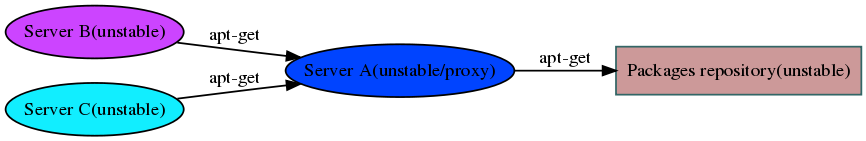
\includegraphics[width=15cm]{image200709/apt-proxy-e.png}
 \end{center}
 \end{figure}

%-------------------------
\subsection{レベル 中}
 一般ユーザーは知っていてもあまり役に立たないと思われる apt-xxx。
\subsubsection{apt-ftparchive}
 Sources.gz / Packages.gz などのパッケージ情報用ファイルを作成するためのツール。
 自分で作ったパッケージを apt-line として公開したいときに使います。
\begin{commandline}
  % apt-ftparchive packages . | gzip -9 > Packages.gz 
  % apt-ftparchive sources . | gzip -9 > Sources.gz
  % apt-ftparchive release . > Release 
\end{commandline}

\subsubsection{apt-sortpkgs}
 Packages ファイル および Sources ファイルをソートします。apt-ftparchive で作成したものはソート
 されていなかったりするので、アルファベット順にソートするときに使います。
\begin{commandline}
 % apt-sortpkgs Packages > Packages.sort
\end{commandline} 

\subsubsection{apt-extracttemplates}
 Debian パッケージから設定とテンプレート情報を抽出するためのツールです。

\begin{commandline}
 % wget http://http.us.debian.org/debian/pool/main/x/xorg/xserver-xorg_7.3~rc1_all.deb
 % apt-extracttemplates xserver-xorg_7.3~rc1_all.deb
 % ls
 xserver-xorg.config.34261
 xserver-xorg.template.34260
\end{commandline}

\subsubsection{apt-build}
 Debian で提供されているバイナリパッケージはあまり最適化されていません。
 人によっては自分の環境に合わせてチューニングしたり、製品に組み込んだりする場合もあります。
 apt-build は apt-get する感覚で環境に合わせてバイナリを作成をサポートするツールです。
 Debian パッケージをリビルドする場合は
 \begin{commandline}
 % apt-get update
 % apt-get source hello
 % cd hello-x.x
 % debuild -us -uc
 % sudo dpkg-i ../hello_xxxx.deb
 \end{commandline}
 という手順を踏みますが、apt-build の場合は
 \begin{commandline}
 % apt-get update
 % apt-build install hello
 \end{commandline}
 だけです。apt-build の設定ファイルは
 \begin{commandline}
 /etc/apt/apt-build.conf
 \end{commandline}
 にあり、
 \begin{commandline}
build-dir = /var/cache/apt-build/build
repository-dir = /var/cache/apt-build/repository
Olevel = -O3
march = -march=pentium2
mcpu = -mcpu=pentium2
options =
 \end{commandline}
 という設定になっています。例えば、自分の使っているマシンが i686 ではなく、Crusoe
 の場合には
\begin{commandline}
Olevel = 
-O2 -fomit-frame-pointer -fno-strict-aliasing -fno-common \ 
-pipe +-mpreferred-stack-boundary=2 -march=i686 -malign-functions=0 \
-malign-jumps=0 -malign-loops=0
\end{commandline}
とすればよいでしょう。

\subsubsection{apt-cross}
 Debian package を cross環境で使用できるように変換してインストールしてます。
 いままでは ダウンロードした Debian package を dpkg-cross で変換して
 インストールしていましたが、apt-cross を使うことのよって、手作業が減らすことが
 できます。

 \begin{figure}[h]
 \begin{center}
apt-cross を使用しない場合
 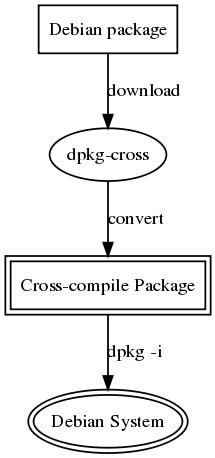
\includegraphics[width=16cm]{image200709/apt-cross.png}
 \end{center}
 \end{figure}

 \begin{figure}[h]
 \begin{center}
apt-cross を使用した場合

 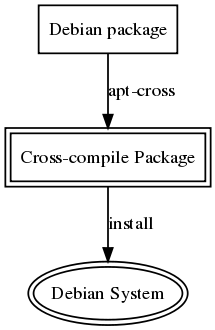
\includegraphics[width=12cm]{image200709/apt-cross-e.png}
 \end{center}
 \end{figure}

\subsubsection{apt-transport-https}
 apt はftp/http で取得できるのですが、このパッケージを使うことによって
 https 経由で apt を行うことができるようになります。
%------------------------- 
\subsection{レベル 高}
 知っていても使わないだろうと思われる apt-xxx.
 話のネタにはなるかもしれない。
\subsubsection{apt-zip}
 リムーバブルメディアの ZIP からの apt をサポートするためのツールです。
 同じようなツールで apt-cdrom がありますが、違いがいまいちわかりません。

\subsubsection{aptsh}
 apt の操作をができる Shell.
\begin{commandline}
 % sudo aptsh
\end{commandline} 
 で shellが aptsh になります。試しに、
\begin{commandline}
 % ls
\end{commandline}
 を実行すると、インストール可能なパッケージ一覧が表示されます。
 
\subsection{まとめ}
今回はさわりだけを説明しました。今回の紹介で気になるapt-xxx がありましたら
詳細を説明していきたいと思っています。

%apt-mirror
%apt-move
%
%apt-watch
%apt-watch-backend
%apt-watch-gnome
%apt-watch-interface

\dancersection{コミックマーケット72の報告}{岩松 信洋}
\label{komike72}
\index{komike72}

東京エリアDebian勉強会および関西エリアDebian勉強会で
作成した資料を本にし、コミックマーケット72で販売をしました。
以下に報告します。

\subsection{イベントについて}
\begin{itemize}
 \item イベント名

	コミックマーケット72
 \item 開催日時

	2007年08月17日から08月19日
 \item 場所

	東京ビックサイト

 \item 出展

	行いませんでした。
 \item 委託先

	美紗緒ネットワークさん \url{http://www.misao.gr.jp/}

	ありがとうございました。
\end{itemize}
\subsection{本の内容}
第23回から第28回までの東京エリア Debian 勉強会資料および一部の関西 Debian 勉強会資料
をまとめ、表紙、奥付を含めて84ページの本を60冊作成しました。

\subsection{印刷代}
\begin{table}
\begin{center}

\begin{tabular}{|c|c|}
\hline
内容 & 金額\\
\hline
表紙代 & 456円\\
\hline
中とじ製本代 & 9000円 \\
\hline
コピー代 & 15840円 \\
\hline
宅配便 & 1500円 \\
\hline
出力手数料 & 600円 \\
\hline\hline
小計 & 27396円 \\
\hline\hline
消費税 & 1369円 \\
\hline\hline
合計 & 28765円 \\
\hline
\end{tabular}
\end{center}
\end{table}

\subsection{販売結果}

\begin{itemize}
	\item 販売金額 

		800円

	\item 販売部数
 
		49部(1冊はサンプルとして提出。)

	\item 売上げ
 
		39200円( 800円*49部 )
\end{itemize}

\subsection{残り}
残りの10冊は関西Debian勉強会用として取りおきしています。

KOF \url{http://k-of.jp/2007/kof.html} や、関西でのイベントなどで
たかやさんに販売して頂くことになっています、

\subsection{次回のコミケ}
コミックマーケット73 が今年の12月29日から31日に開催されます。
次回もどこかに委託していただく予定です。
来年の夏はブースを取って参加したいと考えています。
だれかやる人いませんか?


\dancersection{今後の予定}{岩松 信洋}

\subsection{OSC Tokyo/Fall}
10月5日・6日に開催されます。Debian JP Project も「東京エリアDebian勉強会」として
参加します。OSCでは武藤さんがDebianでの印刷関係についてお話してくれる予定です。
また、10月の勉強会は OSC にて開催したことにします。

%\printindex

\cleartooddpage

\begin{minipage}[b]{0.2\hsize}
 \colorbox{dancerlightblue}{\rotatebox{90}{\fontsize{80}{80} {\gt デビアン勉強会} }}
\end{minipage}
\begin{minipage}[b]{0.8\hsize}

\vspace*{15cm}
{\color{dancerlightblue}\rule{\hsize}{1mm}}
\vspace{2mm}

\includegraphics[width=2cm]{image200502/openlogo-nd.eps}
\noindent \Large \bf Debian 勉強会資料\\ \\
\noindent \normalfont \debmtgyear{}年\debmtgmonth{}月\debmtgdate{}日 \hspace{5mm}  初版第1刷発行\\
\noindent \normalfont 東京エリア Debian 勉強会 (編集・印刷・発行)\\
{\color{dancerdarkblue}\rule{\hsize}{1mm}}
\end{minipage}

\end{document}
